\documentclass[
    12pt
]{article}

\usepackage[
    a4paper,
    left  =2cm,
    right =2cm,
    top   =3cm,
    bottom=3cm,
]{geometry}

\usepackage[
    colorlinks=true,
    linkcolor=blue,
    urlcolor=blue,
]{hyperref}

\usepackage{graphicx}

% \usepackage{xcolor}
\usepackage{minted}
% \usemintedstyle{monokai}
\setminted{
    % bgcolor=black!90,
    linenos,
    tabsize=4,
    breaklines,
    frame=lines,
    fontsize=\footnotesize
}

\title{Digital Image Processing Assignment Report}
\date{\today}
\author{
	Munshi Nishat Alam \\
	ETCE UG4 G1        \\
	002210701061
}

\begin{document}
\maketitle
\tableofcontents

\section{Source Code}
The source code for this report can be found at:
\href{https://github.com/mnaetce/lumina}{lumina}

\subsection{Thirdparty Dependencies}
\begin{itemize}
	\item \textbf{nob.h:}
	      For building the C source code and
	      compiling this \LaTeX{} document
	      (\href{https://github.com/tsoding/nob.h}
	      {tsoding/nob.h}).
	\item \textbf{stb\_image:}
	      For loading and writing images
	      (\href{https://github.com/nothings/stb}
	      {nothings/stb}).
	\item \textbf{raylib:}
	      For visual rendering of images
	      (\href{https://github.com/raysan5/raylib}
	      {raysan5/raylib}).
\end{itemize}

\subsection{Task 1: Contrast Enhancement}
\textbf{Task:} Take an input image that has been acquired in poor light, and hence has poor contrast. Apply a suitable image enhancement algorithm, show the input image and the output image and also include the program in the report.

\subsubsection{Algorithm Used}
Linear Contrast Scaling with $scale = 1.5$

\newpage
\subsection{Input and Output Images}
\begin{figure}[!ht]
	\center
	\includegraphics[width=0.90\linewidth]
	{data/single-fresh-red-strawberry-on-table-green-background-food-fruit-sweet-macro-juicy-plant-image-photo.jpg}
	\caption{Input Image (Poor Contrast)}
	\vspace{1cm}
	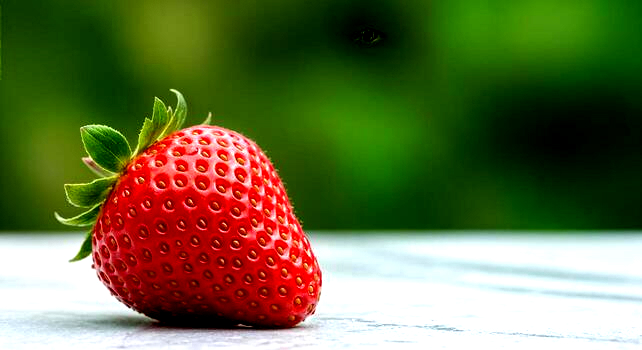
\includegraphics[width=0.90\linewidth]
	{data/single-fresh-red-strawberry-on-table-green-background-food-fruit-sweet-macro-juicy-plant-image-photo.jpg-lumina-enhanced.jpg}
	\caption{Output Image (Enhanced)}
\end{figure}

\newpage
\subsection{C Program (only showing the relevant function)}
\begin{minted}{c}
LuImage lu_enhance(LuImage input)
{
	if (input.channels != 3) {
		nob_log(NOB_ERROR, "We currently only support 3-channel RGB image enchancing");
		exit(1);
	}

	size_t n       = input.width * input.height * input.channels;
	LuImage output = {
		.path     = lu_add_ext(input.path),
		.width    = input.width,
		.height   = input.height,
		.channels = input.channels,
		.data     = calloc(n, sizeof(input.data[0])),
	};

	if (output.data == nullptr) {
		nob_log(NOB_ERROR, "Could not allocate %zu bytes: %s", n, strerror(errno));
		exit(1);
	}

	nob_log(NOB_INFO, "Enhancing %s", input.path);

	for (size_t i = 0; i < n; ++i) {
		// Normalize to [-0.5, 0.5]
		float norm = (float)input.data[i] / 255.0f - 0.5f;

		// scale and clip
		float scale = 1.5f;
		norm *= scale; // [-scale * 0.5, scale * 0.5];
		if (norm < -0.5f) norm = -0.5f;
		if (norm > +0.5f) norm = +0.5f;

		// denormalize and clip
		int byte = (norm + 0.5f) * 255.0f;
		if (byte < 0) byte = 0;
		if (byte > 255) byte = 255;

		// write
		output.data[i] = (stbi_uc)byte;
	}

	return output;
}
\end{minted}

\end{document}
